\chapter{Multi-phase substance models}\label{ch:mp}

Unlike ideal gas properties, it is sensible to formulate multi-phase properties in terms of temperature and density instead of temperature and pressure.  Modeling phase changes with temperature and pressure as independent variables requires a discontinuity at the phase change.  On the other hand, using density requires no such discontinuity, and it even permits modeling meta-stable states.

Historically, there have been countless approaches to the problem, beginning with the so-called ``viral'' terms inspired by Van der Waals forces in early work on the kinetic theory of gases.  This approach began an evolution of increasingly complex variants of the ideal gas law, but parallel models for the specific heat are needed to establish a total substance model.  Eventually, this approach fell out of popularity in favor of single property models from which all other properties could be derived.  

\section{Span and Wagner Equation of State}\label{sec:mp:sweos}

Both the \texttt{mp2} and its predecessor, \texttt{mp1}, use what is sometimes called the ``Span and Wagner'' model.  Its earliest publication appears to be in 1991\cite{stewart:1991, setzmann:1991}, but it was in a three-part paper in 2003 that Span and Wagner make a defense for the model's broad use for the description of the thermodynamic properties of substances across phase change boundaries\cite{span:2003:1, span:2003:2, span:2003:3}. Its most important feature is that it is generalizable to an incredible variety of substances without the need for custom formulae -- all the terms merely need their own coefficients, which a set algorithm can load and use for calculation.  

The models supported by \PM's multi-phase classes uses a single (albeit incredibly complicated) formula for Helmholtz free energy,
\begin{align}
f(T,\rho) &\equiv e(T,\rho) - T s(T,\rho)\\
 &= h - \frac{p}{\rho} - T s.
\end{align}
The model for implementing these models usually goes something like this: Individual researchers accumulate huge bodies of raw experimental data describing the properties like specific heat, pressure, phase-change boundary, critical point, etc.  Then, a team assembles a large bank of terms for an expansion representing $f(T,\rho)$, and iteratively narrows down the model until a minimum number of terms is found that still respects certain error thresholds.  In many cases, the errors are less than the uncertainty in the original data.

\subsection{Nondimensionalization}\label{sec:mp:nd}

These models are almost always published with a nondimensional formulation for free energy.  This means the terms can be scaled to be more or less on the order of unity, and the unit system used in the implementation is irrelevant.  Many authors use $\alpha$ to represent a nondimensional free energy, and we adopt the same here.

All of the substance models in the first multi-phase class use
\begin{subequations}
\begin{align}
\alpha(\tau,\delta) &= \frac{f(T,\rho)}{R T}\\
\tau &= \frac{T_c}{T}\\
\delta &= \frac{\rho}{\rho_c}.
\end{align}
\end{subequations}

The free energy is normalized by the quantity $R T$, which is motivated by (\ref{eqn:ig:efromt}) from the study of ideal gases.  Normalizing temperature and density by the critical point values acknowledges that the critical point is a natural scale for the important phenomena in this substance.  The choice to make $\tau$ scale like the inverse of temperature is motivated by the Boltzmann and Maxwell distributions for molecular velocity, in which temperature appears in a denominator.

The formulation for dimensionless free energy, $\alpha$, is split into two parts: the ideal gas part, $\alpha^o$, and the residual part, $\alpha^r$.  So, the total free energy is
\begin{align}
\alpha(\tau, \delta) = \alpha^o(\tau, \delta) + \alpha^r(\tau, \delta)
\end{align}
This approach separates the problem of needing to model the energy contained in molecular vibration and translation of a large number of independent oscillators ($\alpha^o$) from the problem of modeling the effects of intermolecular forces with increasing density ($\alpha^r$).

\subsection{Ideal gas portion of free energy}\label{sec:mp:ig}
The ideal gas portion of the free energy can be constructed from a specific heat model, just as other properties were for the ideal gas substances in Chapter \ref{ch:ig}.  The ideal gas enthalpy is merely the integral of specific heat, and ideal gas entropy can be similarly constructed in terms of specific heat, temperature, and density,
\begin{subequations}
\begin{align}
h &= h_0 + \int_{T_0}^T c_p \d T\\
s &= s_0 + \int_{T_0}^T \frac{c_p}{T} \d T - R \ln\left(\frac{\rho}{\rho_0}\right) - R\ln\left(\frac{T}{T_0}\right).
\end{align}
\end{subequations}
When these are transposed into the dimensionless parameters, $\tau$ and $\delta$,
\begin{align*}
h &= h_0 - T_c \int_{\tau_0}^\tau \frac{c_p}{\tau^2} \d \tau\\
s &= s_0 - \int_{\tau_0}^\tau \frac{c_p}{\tau} \d \tau - R \ln\left(\frac{\delta \tau_0}{\delta_0 \tau}\right).
\end{align*}
When these are used to calculate the dimensionless free energy,
\begin{align}
\alpha^o &= \frac{h - RT - Ts}{RT} = \frac{h \tau}{R T_c} - 1 - \frac{s}{R}\nonumber\\
 &= \frac{h_0}{RT_c} \tau - \frac{s_0}{R} - 1 + \ln\left(\frac{\delta \tau_0}{\delta_0 \tau}\right) + \left(-\tau\int_{\tau_0}^\tau \frac{c_p}{R \tau^2} \d \tau + \int_{\tau_0}^\tau \frac{c_p}{R \tau} \d \tau \right)\label{eqn:mp:aodef}
\end{align}
Note that, for ease of interpretation, we have adopted a lazy notation with $\tau$ both inside and outside of the integrals.  We will be more strict with our notation below.

The difficulty in formulating the specific heat of even an ideal gas is introduced in Section \ref{sec:intro:e}.  It is, briefly, that portions of energy that a substance stores in translation (thermal energy) versus the many internal forms of vibration depends heavily on the temperature.  A fully detailed model would need to include molecular vibration, electronic, magnetic energies, and quantom mechanical effects.  Within the confines of the Span and Wagner format, different authors are still able to approach this differently -- using formulations that range from polynomial fits to a more physics-based approach.

One of the biggest challenges in describing the specific heats of gases is found at low temperatures.  Here, the different modes of oscillation are found to have dramatically dissimilar energies (defying the equipartition assumption).  The specific heat of many independent oscillators assuming a distribution of discrete energies adopts the form
\begin{align}
\frac{c_p(\tau)}{R} = \ldots + b m^2 \frac{\tau^2 \exp(m\tau)}{\left(\exp(m\tau) - 1\right)^2} + \ldots\nonumber,
\end{align}
where $b$ represents the magnitude of the feature, and $m$ is a dimensionless temperature (normalized by $T_c$) at which the feature occurs.

The integrals of specific heat can be collectively simplified by inverting the integration-by-parts procedure with a series of substitutions, so that
\begin{align}
-\tau \int_{\tau_0}^\tau \frac{c_p(t)}{Rt^2} \d t + \int_{\tau_0}^\tau \frac{c_p(t)}{Rt} \d t = - \int_{\tau_0}^\tau \left[ \int_{\tau_0}^t \frac{c_p(t')}{Rt'^2} \d t'\right] \d t.
\end{align}
This has the fortunate effect of canceling the $\tau^2$ in the quantum component of specific heat, making its integral straightforward.
\begin{align}
-\int_{\tau_0}^\tau &\int_{\tau_0}^t \frac{b m^2 \exp(m t')}{\left(\exp(m t') - 1\right)^2} \d t' \d t  \ldots\nonumber\\
 &= \int_{\tau_0}^\tau \left[ \frac{b m}{\exp(m t) - 1} - \frac{b m}{\exp(m \tau_0) - 1} \right] \d t \nonumber\\
 &= \int_{\tau_0}^\tau \frac{b m\exp(-mt)}{1 - \exp(-mt)}\d t - \frac{b m}{\exp(m\tau_0)-1}(\tau - \tau_0) \nonumber\\
 &= b\ln(1-\exp(-m\tau)) - b\ln(1-\exp(-m\tau_0)) + \ldots\nonumber\\
 & \hspace{2em} -\frac{b m}{\exp(m\tau_0)-1}(\tau - \tau_0)
\end{align}

The same approach could be applied to the integration of the polynomial, but it is probably more easily dealt with in separate terms.  For a sum of terms with arbitrary exponents,
\begin{align}
-\tau \int_{\tau_0}^\tau &\sum_k c_k t^{k-2} \d t + \int_{\tau_0}^\tau \sum_k c_k t^{k-1} \d t \ldots \nonumber\\
&= -\tau \left[c_1 \ln t + \sum_{k\ne 1} \frac{c_k t^{k-1}}{k-1} \right]_{\tau_0}^\tau  + \left[c_0 \ln t + \sum_{k\ne 0} \frac{c_k t^{k}}{k} \right]_{\tau_0}^\tau\nonumber\\
&= - \tau c_1 \ln \tau + \tau c_1 \ln \tau_0 - \left[\sum_{k\ne 1} \frac{c_k \tau^k}{k-1}\right] + \tau \left[\sum_{k\ne 1} \frac{c_k \tau_0^{k-1}}{k-1} \right] + \ldots\nonumber\\
&\hspace{2em}  + c_0 \ln \tau - c_0 \ln \tau_0 + \left[ \sum_{k\ne 0} \frac{c_k \tau^{k}}{k} \right] - \left[ \sum_{k\ne 0} \frac{c_k \tau_0^{k}}{k} \right].
\end{align}
Note that this analysis does not require that values of $k$ be limited to integers.

Collectively, these integrals motivate the form that is now commonplace in contemporary free-energy-based models,
\begin{subequations}
\begin{align}
\alpha^o(\tau,\delta) = \ln \delta + (c_0 + c_1\tau) \ln \tau + \alpha^o_0(\tau) + \alpha^o_1(\tau),\label{eqn:mp:ao}
\end{align}
where $\alpha^o_0$ is a polynomial on $\tau$,
\begin{align}
\alpha^o_0(\tau) = \sum_k c_j \tau^k \label{eqn:mp:ao:0},
\end{align}
and $\alpha^o_1$ includes the quantum terms,
\begin{align}
\alpha^o_1(\tau) = \sum_j b_j \ln\left(1 - \exp( -m_j \tau ) \right)\label{eqn:mp:ao:1}.
\end{align}
\end{subequations}

In many models, the $\tau \ln \tau$ term is omitted from Equation \ref{eqn:mp:ao}, implying that there was no linear term on $\tau$ (proportional to $1/T$) in the formulation of specific heat.  Because much of the complexity of the specific heat is captured by the $\alpha^o_1$ terms, the polynomial, $\alpha^o_0$, may only contain a constant and a linear term.  Still, exponentials and logarithms are numerically expensive, so this model is usually substantially slower than the polynomial ideal gas models.


\subsection{Residual portion of free energy}
The residual (or real-fluid) portion of free energy attempts to account for everything that the ideal gas portion does not.  Many of these terms become especially important when the substance density is high, because intermolecular forces are specifically ignored in the ideal gas model.  The model is divided into three groups of terms,
\begin{subequations}
\begin{align}
\alpha^r &= \alpha^r_0(\tau, \delta) + \alpha^r_1(\tau, \delta) + \alpha^r_2(\tau, \delta)\label{eqn:mp:ar}
\end{align}
Many of these terms are physically motivated, but that discussion is not included here.

The first group of terms is a series of polynomials multiplied by exponentials of powers of density,
\begin{align}
\alpha^r_0 &= p_0(\tau, \delta) + \sum_{k=1}^K \exp\left(-\delta^k\right) p_k(\tau, \delta)\\
& p_k = \sum_i c_i \tau^{a_i} \delta^{b_i}.\label{eqn:mp:ar0}
\end{align}
While it is not explicitly forbidden, the $\delta$ exponent, $b$, is neither zero nor negative in these models, so $\alpha^r_0$ terms with the exponential multipliers vanish near $\delta \rightarrow 0$ and $\delta \rightarrow \infty$.  These terms model the complicated behaviors that occur near the phase change (when $\delta$ is on the order 1).

In most models, the first group ($\alpha^r_0$) constitutes the largest number of terms (often dozens).  The exponents in the polynomial expansion are sometimes integers, but they are often rationals (which permits efficient evaluation using the method described in Section \ref{sec:num:poly2}), and they are rarely long decimal values.  

The second group of terms, $\alpha^r_1$, is a Gaussian function multiplied by polynomial terms of $\tau$ and $\delta$.  It was first introduced in 1991 by Setzmann et al. to better model the severely distorted surface that occurs near the critical point in oxygen.  Most models only use a few of these terms at most, and they are usually centered (by $\epsilon$ and $\gamma$) very close to the critical point.  From the 1991 paper, ``The opinion has been widely held that analytic equations of state covering the whole fluid region are not able to represent the properties in the critical region.'' The authors continue to say, ``We will show that our new equation is
able to represent the existing experimental information on the thermodynamic properties of methane in the critical
region at least as well as [competing models].'' \cite{setzmann:1991}

The third group, $\alpha^r_2$, is a Gaussian centered on exactly the critical point, but the coefficient, $\Delta$, is a scaled distance from the critical point.  The term appears in a 1994 paper modeling carbon dioxide \cite{span:1994} and again in a 2014 revision to the properties of water and steam \cite{iapws:2014}, but in conspicuously few others.  While its formulation is not explained in detail in these sources, it allows for a more complicated shape from the term without the computational expense of additional polynomial terms.  It seems to have been designed to reduce the number of Gaussian terms required to produce the desired result at the critical point.

\begin{align}
\alpha^r_1 &= \sum_{l=0}^L c_l \delta^{d_l} \tau^{t_l} \exp\left( -a_l(\delta-\epsilon_l)^2 - b_l(\tau-\gamma_l)^2 \right)\label{eqn:mp:ar1}\\
\alpha^r_2 &= \sum_{m=0}^M c_m \Delta_m{^{b_m}} \delta \exp\left(-C_m(\delta-1)^2 - D_m(\tau-1)^2 \right)\label{eqn:mp:ar2}\\
 &\Delta_m = \left[1-\tau + A_m\left((\delta-1)^2\right)^{1/2\beta_m} \right]^2 + B_m\left((\delta - 1)^2\right)^{a_m}.
\end{align}
\end{subequations}
At first glance, these formulations may appear to be an inefficient tangled mess of nested exponents.  However, quantities like $\tau-1$ and $\delta-1$ may be positive or negative, and the exponents are not integers.  It is numerically elegant to square these quantities (requiring just a multiplication operation) before raising them to decimal or fractional powers.

\subsection{Derivatives of free energy}

As we will address in the next section, it is also important to evaluate up to the second derivative of these terms.  This is sufficiently cumbersome to deserve some treatment here.  The efficient evaluation of derivatives of polynomials is addressed in Section \ref{sec:num:poly2}, so we only need to treat the other aspects of these functional forms.

The ideal gas portion in (\ref{eqn:mp:ao}) has derivatives
\begin{subequations}
\begin{align}
\alpha^o_\tau &= (c_0-1)\tau^{-1} + c_1 (1 + \ln \tau) + \alpha^o_{0,\tau} + \alpha^o_{1,\tau}\\
\alpha^o_\delta &= \delta^{-1}\\
\alpha^o_{\tau\tau} &= -(c_0-1)\tau^{-2} + c_1 \tau^{-1} + \alpha^o_{0,\tau\tau} + \alpha^o_{1,\tau\tau}\\
\alpha^o_{\tau\delta} &= 0\\
\alpha^o_{\delta\delta} &= -\delta^{-2}
\end{align}
\end{subequations}
The polynomial, $\alpha^o_0(\tau)$, and its derivatives can be evaluated separately.  All that remains is to determine the derivatives of $\alpha^o_1(\tau)$.

\begin{subequations}
\begin{align}
\alpha^o_{1,\tau} &= \sum_j \frac{b_j m_j}{\exp(m_j \tau) - 1}\\
\alpha^o_{1,\tau\tau} &= \sum_j \frac{b_j m_j^2 \exp(m_j \tau)}{(\exp(m_j \tau) - 1)^{2}}
\end{align}
\end{subequations}

Derivatives of the residual portion in (\ref{eqn:mp:ar}) can be calculated individually.  Much of $\alpha^r_0$ in (\ref{eqn:mp:ar0}) can be calculated trivially from the derivatives of the polynomials. 
\begin{subequations}
\begin{align}
\alpha^r_{0,\tau} &= p_{0,\tau} + \sum_{k=1}^K \exp\left( -\delta^k \right) p_{k,\tau}\\
\alpha^r_{0,\delta} &= p_{0,\delta} + \sum_{k=1}^K \exp\left(-\delta^k\right) \left(p_{k,\delta} - k \delta^{k-1} p_k\right)\\
\alpha^r_{0,\tau\tau} &= p_{0,\tau\tau} + \sum_{k=1}^K \exp\left( -\delta^k \right) p_{k,\tau\tau}\\
\alpha^r_{0,\tau\delta} &= p_{0,\tau\delta} + \sum_{k=1}^K \exp\left(-\delta^k\right) \left(p_{k,\tau\delta} - k \delta^{k-1} p_{k,\tau}\right)\\
\alpha^r_{0,\delta\delta} &= p_{0,\delta\delta} + \sum_{k=1}^K \exp\left(-\delta^k\right) \left(p_{k,\delta\delta} -k(k-1) \delta^{k-2} p_{k} \right. \ldots\nonumber\\
 &\left. \hspace{2em} - 2k\delta^{k-1}p_{k,\delta} +  k^2 \delta^{2(k-1)} p_k\right)
\end{align}
\end{subequations}

Derivatives of the first Gaussian terms in (\ref{eqn:mp:ar1}) are conveniently calculated as proportional to the terms themselves.  If each term were expressed as the polynomial term multiplier, $p_l$, and the Gaussian term, $g_l$, then $\alpha^r_1 = \sum_l p_l g_l$.  Derivatives on $\alpha^r_1$ can be conveniently constructed in terms of those intermediates.
\begin{subequations}
\begin{align}
p_l &= c_l\ \tau^{t_l} \delta^{d_l}\\
p_{l,\tau} &= t_l \frac{p_l}{\tau}\\
p_{l,\delta} &= d_l \frac{p_l}{\delta}\\
p_{l,\tau\tau} &= t_l(t_l-1) \frac{p_l}{\tau^2}\\
p_{l,\tau\delta} &= t_l d_l \frac{p_l}{\tau\delta}\\
p_{l,\delta\delta} &= d_l (d_l-1) \frac{p_l}{\delta^2}
\end{align}
\end{subequations}
\begin{subequations}
\begin{align}
g_l &= \exp\left( -a_l(\delta-\epsilon_l)^2 - b_l (\tau-\gamma_l)^2 \right)\\
g_{l,\tau} &= -2 b_l (\tau - \gamma_l)\ g_l\\
g_{l,\delta} &= -2 a_l (\delta - \epsilon_l)\ g_l\\
g_{l,\tau\tau} &= -2 b_l\ g_l - 2 b_l (\tau - \gamma_l)\ g_{l,\tau}\\
g_{l,\tau\delta} &= -2 b_l (\tau - \gamma_l)\ g_{l,\delta} = -2 a_l (\delta - \epsilon_l)\ g_{l,\tau}\\
g_{l,\delta\delta} &= -2 a_l\ g_l - 2 a_l (\delta - \epsilon_l)\ g_{l,\delta}
\end{align}
\end{subequations}

\begin{subequations}
\begin{align}
\alpha^r_{1,\tau} &= \sum^L_{l=0} p_{l,\tau}\ g_l + p_l\ g_{l,\tau}\\
\alpha^r_{1,\delta} &= \sum^L_{l=0} p_{l,\delta}\ g_l + p_l\ g_{l,\delta}\\
\alpha^r_{1,\tau\tau} &= \sum^L_{l=0} p_{l,\tau\tau}\ g_l + 2 p_{l,\tau}\ g_{l,\tau} + p_l\ g_{l,\tau\tau}\\
\alpha^r_{1,\tau\delta} &= \sum^L_{l=0} p_{l,\tau\delta}\ g_l + p_{l,\tau}\ g_{l,\delta} + p_{l,\delta}\ g_{l,\tau} + p_l\ g_{\tau\delta}
\end{align}
\end{subequations}

This approach to evaluating derivatives in stages helps numerical efficiency, since there are obvious ways to make repeated use of intermediate values, but it also helps with the clarity of the code.  The same approach is even more valuable in the treatment of the second Gaussian terms in (\ref{eqn:mp:ar2}).  First, we turn our attention to derivatives of the distance term, $\Delta$.  For ease of notation, we will omit the subscript, $m$, on all of the empirical coefficients.
\begin{subequations}
\begin{align}
\Delta_\tau &= -2\left[ 1 - \tau + A\left((\delta-1)^2 \right)^{1/2\beta} \right]\\
\Delta_\delta &= 2 \frac{A}{\beta} \left[ 1 - \tau + A\left((\delta-1)^2 \right)^{1/2\beta} \right] \left((\delta-1)^2 \right)^{1/2\beta - 1/2}\\
\Delta_{\tau\tau} &= 2\\
\Delta_{\tau\delta} &= 2\frac{A}{\beta}\left((\delta-1)^2 \right)^{1/2\beta - 1/2}\\
\Delta_{\delta\delta} &= 2\left(\frac{A}{\beta}\right)^2 \left((\delta-1)^2\right)^{1/\beta-1} \ldots \nonumber\\
& + 2\frac{A}{\beta}\left(\frac{1}{\beta} - 1\right) \left[ 1 - \tau + A\left((\delta-1)^2 \right)^{1/2\beta} \right] \left((\delta-1)^2 \right)^{1/2\beta - 1}
\end{align}
\end{subequations}

Next, we will consider the exponential term separately,
\begin{subequations}
\begin{align}
f(\tau, \delta) &= \exp(-C (\delta-1)^2 - D(\tau-1)^2)\\
f_\tau &= -2D(\tau-1) f\\
f_\delta &= -2C(\delta-1) f\\
f_{\tau\tau} &= -2D f - 2D(\tau-1) f_\tau\\
f_{\tau\delta} &= -2D(\tau-1) f_\delta = -2C(\delta-1) f_\tau\\
f_{\delta\delta} &= -2C f - 2C(\delta-1) f_\delta
\end{align}
\end{subequations}

Finally, the $\alpha_2^r$ derivatives may be constructed as
\begin{subequations}
\begin{align}
\alpha^r_2 &= \Delta^b \delta f\\
\alpha^r_{2,\tau} &= b \Delta_\tau \Delta^{b-1} \delta f + \Delta^b \delta f_\tau\\
\alpha^r_{2,\delta} &= b \Delta_\delta \Delta^{b-1} \delta f + \Delta^b f + \Delta^b \delta f_\delta\\
\alpha^r_{2,\tau\tau} &= b\left( \Delta_{\tau\tau} \Delta^{b-1} + (b-1)\Delta_\tau{^2}\Delta^{b-2} \right) \delta f \ldots  \nonumber\\
 &\hspace{2em} + 2 b \Delta_\tau \Delta^{b-1} \delta f_{\tau} + \Delta^b \delta f_{\tau\tau}\\
\alpha^r_{2,\tau\delta} &= b \left(\Delta_{\tau\delta} \Delta^{b-1} + (b-1)\Delta_\tau \Delta_\delta \Delta^{b-2} \right) \delta f \ldots\nonumber\\
 &\hspace{2em} + b\Delta_{\tau} \Delta^{b-1} f + \Delta^b f_\tau + \ldots \nonumber\\
 &\hspace{2em} + b\Delta_{\tau} \Delta^{b-1} \delta f_\delta + \Delta^b \delta f_{\tau\delta}\\
\alpha^r_{2,\delta\delta} &= b \left(\Delta_{\delta\delta} \Delta^{b-1} + (b-1)\Delta_\delta{^2} \Delta^{b-2} \right) \delta f \ldots\nonumber\\
 &\hspace{2em} + b\Delta_{\delta} \Delta^{b-1} f + \Delta^b f_\delta + \ldots \nonumber\\
 &\hspace{2em} + b\Delta_{\delta} \Delta^{b-1} \delta f_\delta + \Delta^b \delta f_{\delta\delta}
\end{align}
\end{subequations}

\section{Calculation of properties}\label{sec:mp1:properties}

The \texttt{mp1} class calculates all substance properties from temperature, density, $\alpha$, and its derivatives.  In this section, the formulae that are used to calculate the various properties are developed from first principles.

In this development, it will be useful to have this form of the first law:
\begin{align}
T\d s &= \d e - \frac{p}{\rho^2} \d \rho\label{eqn:mp:law1}.
\end{align}

By definition,
\begin{align}
f &= e - Ts \label{eqn:mp:f}.
\end{align}
Its derivatives with respect to temperature and density may be simplified with some help from (\ref{eqn:mp:law1}),
\begin{align}
\left(\frac{\partial f}{\partial T}\right)_\rho &= \left(\frac{\partial e}{\partial T}\right)_\rho - s - T \left(\frac{\partial s}{\partial T}\right)_\rho &=& \ -s\label{eqn:mp:ft}\\
\left(\frac{\partial f}{\partial \rho}\right)_T &= \left(\frac{\partial e}{\partial \rho}\right)_T - T \left(\frac{\partial s}{\partial \rho}\right)_T &=& \ \frac{p}{\rho^2} \label{eqn:mp:fd}.
\end{align}

The properties below are calculated in a dimensionless form.  In this way, this document is relieved from needing to be sensitive to units -- including molar versus mass. 
 
\subsection{Pressure}\label{sec:mp1:p}

The pressure (and compressibility factor) can be calculated explicitly from (\ref{eqn:mp:fd}),
\begin{align}
\frac{p}{\rho R T} &=  \frac{\rho}{R T}\left(\frac{\partial f}{\partial \rho}\right)_T\nonumber\\
&= \delta \alpha_\delta\label{eqn:mp:p}.
\end{align}

\subsection{Entropy}\label{sec:mp1:s}

Entropy appears explicitly in (\ref{eqn:mp:ft}), so it only needs to be transformed into terms of $\alpha$.  First, it is helpful to observe that derivatives with respect to temperature may be transposed into derivatives with respect to $\tau$ 
\begin{align}
\frac{\partial}{\partial T} = -\frac{\tau}{T} \frac{\partial}{\partial \tau}.\nonumber
\end{align}
Therefore, 
\begin{align}
s &= -\left(\frac{\partial f}{\partial T}\right)_\rho \nonumber\\
&= -\frac{\partial}{\partial T} R T \alpha\nonumber\\
&= -R \alpha + R \tau \alpha_\tau
\end{align}
So, normalized by $R$, entropy is
\begin{align}
\frac{s}{R} = \tau \alpha_\tau - \alpha\label{eqn:mp:s}
\end{align}

\subsection{Internal energy}\label{sec:mp1:e}

Internal energy can be calculated in terms of $a$ and $s$ from (\ref{eqn:mp:f}) and (\ref{eqn:mp:s}),
\begin{align}
\frac{e}{R T} &= \frac{f}{RT} + \frac{s}{R} \vspace{2em} =\ \tau \alpha_\tau\label{eqn:mp:e}.
\end{align}

\subsection{Enthalpy}\label{sec:mp1:h}

Enthalpy is trivial to construct from (\ref{eqn:mp:p}) and (\ref{eqn:mp:e}).  By definition, 
\begin{align}
\frac{h}{R T} &= \frac{e}{RT} + \frac{p}{\rho R T}\nonumber\\
 &= \tau \alpha_\tau + \delta \alpha_\delta.\label{eqn:mp:h}
\end{align}

\subsection{Gibbs free energy}\label{sec:mp1:g}

Gibbs' energy is readily calculated from enthalpy and entropy; or from Helmholtz free energy.
\begin{align}
\frac{g}{R T} &= \frac{h}{RT} - \frac{s}{R} = \frac{f}{RT} + \frac{p}{\rho RT}\nonumber\\
&= \alpha + \delta \alpha_\delta.
\end{align}

\subsection{Specific heats}\label{sec:mp1:c}

Constant-volume specific heat is obtained by differentiating internal energy by temperature.
\begin{align*}
c_v &= \frac{\partial e}{\partial T} = e_\tau \frac{\d \tau}{\d T}\\
 &= -e_\tau \frac{\tau}{T}
\end{align*}
From (\ref{eqn:mp:e}), $e$ is simply $R T_c \, \alpha_\tau$, so
\begin{align}
\frac{c_v}{R} = - \tau^2 \alpha_{\tau\tau}\label{eqn:mp:cv}.
\end{align}

Constant-pressure specific heat is not so simply obtained since pressure is not one of the independent variables of the formulation.  Derivations for $c_p$ usually begin with enthalpy, but it will become aparent that the calculation benefits from the prior derivation for $c_v$.  Therefore, from (\ref{eqn:intro:1stlaw}) we may write
\begin{align*}
c_p &= \left(\frac{\partial e}{\partial T}\right)_p - \frac{p}{\rho^2} \left(\frac{\partial \rho}{\partial T}\right)_p.
\end{align*}

However, because the \texttt{mp1} formulation is always in terms of temperature and density, derivatives with constant pressure must be transposed to derivatives on $T$ and $\rho$, 
\begin{align*}
\left(\frac{\partial e}{\partial T}\right)_p &=  \left(\frac{\partial e}{\partial T}\right)_\rho +  \left(\frac{\partial e}{\partial \rho}\right)_T  \left(\frac{\partial \rho}{\partial T}\right)_p.
\end{align*}
Of course, the same must be done for the derivative of density,
\begin{align*}
\left(\frac{\partial \rho}{\partial T}\right)_p &= -\frac{ \left(\frac{\partial p}{\partial T}\right)_\rho }{ \left(\frac{\partial p}{\partial \rho}\right)_T }.
\end{align*}
Substituting,
\begin{align*}
c_p &= \left(\frac{\partial e}{\partial T}\right)_\rho - \left(\left(\frac{\partial e}{\partial \rho}\right)_T - \frac{p}{\rho^2}\right) \frac{ \left(\frac{\partial p}{\partial T}\right)_\rho }{ \left(\frac{\partial p}{\partial \rho}\right)_T }.
\end{align*}
The first term (the derivative of interneral energy with respect to temperature) is merely $c_v$.  The second term may be simplified using (\ref{eqn:mp:law1}), so
\begin{align*}
c_p &= c_v - T\left(\frac{\partial s}{\partial \rho}\right)_T \frac{ \left(\frac{\partial p}{\partial T}\right)_\rho }{ \left(\frac{\partial p}{\partial \rho}\right)_T }.
\end{align*}

Finally, this is in a form that can be conveniently substituted for free energy.  Using (\ref{eqn:mp:ft}) and (\ref{eqn:mp:fd}),
\begin{align*}
\left(\frac{\partial s}{\partial \rho}\right)_T &= - \frac{\partial^2 f}{\partial T \partial \rho} = - \frac{R}{\rho}\left( \delta \alpha_\delta - \tau \delta \alpha_{\tau\delta} \right)\\
\left(\frac{\partial p}{\partial T}\right)_\rho &= \rho^2 \frac{\partial^2 f}{\partial T \partial \rho} = R \rho \left( \delta \alpha_\delta - \tau \delta \alpha_{\tau\delta} \right)\\
\left(\frac{\partial p}{\partial \rho}\right)_T &= 2 \rho \left(\frac{\partial f}{\partial \rho}\right)_T + \rho^2 \left(\frac{\partial^2 a}{\partial \rho^2}\right)_T \ldots\\
 &= RT \left( 2\delta \alpha_\delta + \delta^2 \alpha_{\delta\delta} \right)
\end{align*}
So, 
\begin{align}
\frac{c_p}{R} = \frac{c_v}{R} + \frac{\left(\delta \alpha_\delta - \tau \delta \alpha_{\tau\delta} \right)^2}{2\delta \alpha_\delta + \delta^2\alpha_{\delta\delta}}
\end{align}


\subsection{Speed of sound}

From its definition in Section \ref{sec:intro:a}, we write a dimensionless speed of sound
\begin{align}
\frac{a^2}{R T} &= \frac{1}{RT} \left(\frac{\partial p}{\partial \rho}\right)_s\nonumber\\
  &= \frac{1}{RT} \left(\frac{\partial p}{\partial \rho}\right)_T + \frac{1}{RT} \left(\frac{\partial p}{\partial T}\right)_\rho\left(\frac{\partial T}{\partial \rho}\right)_s. \label{eqn:mp:a0}
\end{align}

The first term is obtained by differentiating (\ref{eqn:mp:p}) with respect to density, producing
\begin{align}
\frac{1}{RT} \left(\frac{\partial p}{\partial \rho}\right)_T &= 2 \delta \alpha_\delta + \delta^2 \alpha_{\delta\delta}
\end{align}

The second term in (\ref{eqn:mp:a0}), we further sub-divide into two parts.  The first part is also obtained by differentiating (\ref{eqn:mp:p}), giving
\begin{align}
\left(\frac{\partial p}{\partial T}\right)_\rho = \rho R (\delta \alpha_\delta - \tau \delta \alpha_{\tau \delta}).
\end{align}
The second part involves the heating of the substance due to its isentropic compression.  For this, we turn to 
\begin{align*}
0 = T \d s = \d e - \frac{p}{\rho^2}\d \rho.
\end{align*}
When we substitute (\ref{eqn:mp:e}) for $e$ and (\ref{eqn:mp:p}) for $p/\rho$, we obtain
\begin{align*}
0 &= -R \tau^2 \alpha_{\tau\tau} \d T + \frac{R T_c}{\rho_c} \alpha_{\tau\delta} \d \rho - \frac{RT}{\rho} \delta \alpha_\delta \d \rho
\end{align*}
Solving for $\d T / \d \rho$, we obtain
\begin{align}
\left(\frac{\partial T}{\partial \rho}\right)_s = -\frac{T}{\rho}\frac{\delta\alpha_\delta - \tau\delta\alpha_{\tau\delta}}{\tau^2 \alpha_{\tau\tau}}
\end{align}

Finally, the dimensionless speed of sound is
\begin{align}
\frac{a^2}{RT} &= 2\delta \alpha_\delta + \delta^2 \alpha_{\delta\delta} - \frac{(\delta \alpha_\delta - \tau\delta \alpha_{\tau\delta})^2}{\tau^2\alpha_{\tau\tau}}.\label{eqn:mp:a}
\end{align}

\subsection{Liquid-vapor line}

The Maxwell criteria provide a means for calculated the saturation line from a substance's properties -- the two phases will be at the same temperature, pressure, and their Gibbs energy is equal.  So,
\begin{subequations}
\begin{align}
g(T,\rho_L) &= g(T,\rho_V)\label{eqn:mp:maxwellg}\\
p(T,\rho_L) &= p(T,\rho_V)\label{eqn:mp:maxwellp},
\end{align}
\end{subequations}
where $\rho_V$ and $\rho_L$ are the vapor and liquid densities respectively.

For Newton-like numerical iteration algorithms, it is essential to provide reasonable initial guesses for $\rho_L$ and $\rho_V$.  Careless guesses can simply result in $\rho_L = \rho_V$, which is a classic example of a computer solution being \emph{not wrong} but not helpful.  The worst case, especially problematic near the critical point, is divergence.


\section{The multi-phase collection}

In \PM, the Span and Wagner models are implemented in classes \texttt{mp1} and \texttt{mp2}.  Because these classes are different implementations of the same model, they use the same data file structure.  See Section \ref{ch:regdat:data} for more information on \PM\ data.

\subsection{The model coefficients}

As of version 3.0.1, all multi-phase data sets contain ideal gas terms in a dictionary called the \texttt{"IGgroup"}.  An \texttt{"IGgroup"} entry in the file might appear like the example below.  The temperature and density scales are simply scalars, and they are expected (but not required) to be equal to the critical density and temperature.  The \texttt{logt} and \texttt{tlogt} entries are also scalar coefficients for their respective terms in Equation \ref{eqn:mp:ao}, but if they are omitted, they are presumed zero.  The \texttt{coef0} is required to be a polynomial definition, as described in Section \ref{sec:num:poly1}.  The \texttt{coef1} value is expected to be a list of two-element lists or tuples used to define the quantum terms in Equation \ref{eqn:mp:ao:1}.

% This comment numbers the code columns.  There are 53 before a line overrun.
%        1         2         3         4         5
%2345678901234567890123456789012345678901234567890123
\begin{lstlisting}[language=Python]
"IGgroup" : {
    "logt" : <c0>,
    "tlogt" : <c1>,
    "group0" : <polynomial definition>,
    "group1" : [[<m0>, <b0>], [<m1>, <b1>], <...>]
}
\end{lstlisting}

The residual coefficients are contained in a similar dictionary called \texttt{"Rgroup"}.  The \texttt{coef0} member contains a list of 2D polynomials (see Section \ref{sec:num:poly2}).  Each a polynomial, $p_k$, corresponds to an exponential term, $\exp(-\delta^k) p_k(\tau, \delta)$.  They are listed in order, so the first polynomial definition corresponds to $k=0$, the second to $k=1$, and so on.  The \texttt{coef1} and \texttt{coef2} members are nested lists with each containing the necessary coefficients and exponents to construct the terms of $\alpha^r_1$ and $\alpha^r_2$ respectively.  
% This comment numbers the code columns.  There are 53 before a line overrun.
%        1         2         3         4         5
%2345678901234567890123456789012345678901234567890123
\begin{lstlisting}[language=Python]
"Rgroup" : {
  "group0" : [<p0>, <p1>, ...]
  "group1" : [
    [<t>, <d>, <b>, <a>, <gamma>, <epsilon>, <c>],
      ...    ]
  "group2" : [
    [<a>, <b>, <beta>, <A>, <B>, <C>, <D>, <c>], 
      ...    ]
}
\end{lstlisting}

\subsection{The \texttt{mp2} class}

The \texttt{mp2} class is the newer of the two multi-phase classes, first implemented in version 3.0.1.  It has a number of powerful advantages over the \texttt{mp1} class
\begin{itemize}
\item For the vast majority of user cases, it is significantly faster.
\item It extends property specification to nearly all valid input combinations.
\item The free energy model coefficients and the critical points are the only information required -- no saturation curves are needed.
\item The algorithms in \texttt{mp2} eliminate the possibility for redundant contradictory information -- all numerical calculations have a single authoritative source data set.
\end{itemize}

The last item is a nuanced, but very important idea.  In \texttt{mp1}, the critical temperature, density, and pressure are all specified, along with models for the saturation lines.  However, those data are all redundant with the thermodynamic model, since they can also be calculated explicitly (albeit very slowly) from the model.  Though \texttt{mp1}'s design improves its performance, it creates strange edges cases, where slightly contradictory saturation properties can be calculated, for the same state, depending on the method used.  A big part of \texttt{mp2}'s design is eliminating those problems without sacrificing speed.

When a \texttt{mp2} instance is retrieved with \texttt{get()} and every time a property is evaluated, the \verb|mp2._build()| method is called to verify that the substance's tables have been calculated.  The process takes some computation time, so it is not performed on all substances -- only those called up for use.  If necessary, the \verb|_build()| method calls (in strict order) \verb|_build_sattab()| then \verb|_build_tab()|, which create dictionary attributes \verb|_sattable| and \verb|_table| respectively.  These lookup tables are central to the algorithm's speed and superior numerical stability.  For any iterative calculation, the tables provide initial guesses very close to the correct state.  As a result, even the most difficult calculations usually converge in only two or three standard Newton-Rhapson iterations.

\textbf{Constructing the saturation table} is the first and slowest part of table construction.  After initialization, the \texttt{mp2} instance has no information on its saturation properties -- only its critical temperature and density and the triple point temperature.  Especially near the critical point, guesses need to be extremely near to their actual values, lest they diverge, so \verb|_build_sattab()| calculates the table one point at a time.  Once a point on the saturation curve converges, its local derivatives are used to extrapolate to the next point a small step away.

Derivatives are calculated from the Maxwell criteria in Equations \ref{eqn:mp:maxwellg} and \ref{eqn:mp:maxwellp}.  These represent two constraints with three variables, $T$, $\rho_L$, and $\rho_V$, so the tangent to the curve they form in 3-space can be calculated from their derivatives.  For ease of notation,
\begin{subequations}
\begin{align}
g_{L,T} &= \frac{\partial g(T, \rho_L)}{\partial T}\\
g_{L,\rho} &= \frac{\partial g(T, \rho_L)}{\partial \rho}\\ 
p_{L,T} &= \frac{\partial p(T, \rho_L)}{\partial T}\\
p_{L,\rho} &= \frac{\partial p(T, \rho_L)}{\partial \rho}
\end{align}
\end{subequations}
The derivatives of the Maxwell criteria are, therefore,
\begin{subequations}
\begin{align}
g_{L,T}\, \d T + g_{L,\rho}\, \d \rho_L &= g_{V,T}\, \d T + g_{V,\rho}\, \d \rho_V\\
p_{L,T}\, \d T + p_{L,\rho}\, \d \rho_L &= p_{V,T}\, \d T + p_{V,\rho}\, \d \rho_V.
\end{align}
\end{subequations}

It is possible to calculate the differential of any two of the variables in terms of the third.  For example, with respect to temperature,
\begin{align}
\left[\begin{array}{cc}
g_{L,\rho} & -g_{V,\rho}\\
p_{L,\rho} & -p_{V,\rho}
\end{array}\right]  \left[\begin{array}{c}
\d \rho_L \\
\d \rho_V
\end{array}\right] = 
\left[\begin{array}{c}
-g_{L,T} + g_{V,T} \\
-p_{L,T} + p_{V,T}
\end{array}\right] \d T
\end{align}
and finally
\begin{align}
\Delta &= -g_{L,\rho} p_{V,\rho} + g_{V,\rho} p_{L,\rho}\\
\frac{\d \rho_L}{\d T} &= \frac{1}{\Delta}\big[(g_{L,T}-g_{V,T}) p_{V,\rho} + (-p_{L,T}+p_{V,T}) g_{V,\rho}  \big]\\
\frac{\d \rho_V}{\d T} &= \frac{1}{\Delta}\big[(g_{L,T}-g_{V,T}) p_{L,\rho} + (-p_{L,T}+p_{V,T}) g_{L,\rho}  \big]
\end{align}

Unfortunately, very near the critical point, these derivatives become singular, since all of the properties (and their derivatives) are very nearly equal.  The problem is yet worse, because the saturation curve is tangent to a line of constant temperature near the critical point.  To avoid this problem, \verb|_build_sattab()| uses similar derivatives with respect to vapor density, $\d T / \d \rho_V$ and $\d \rho_L / \d \rho_V$ instead, and transitions back to temperature far from the critical point.

To keep the tabulated points very nearly equally spaced throughout the table, the ``distance'' to the next saturation point is scaled by the metric
\begin{align}
0.02 = \sqrt{\left(\frac{\Delta T}{T_c}\right)^2 + \left(\frac{\Delta \rho_V}{\rho_c}\right)^2 + \left(\frac{\Delta \rho_L}{\rho_c}\right)^2}.
\end{align}
The ``deltas'' are rescaled in proportion to force the ``step'' size to be 0.02.  Depending on the substance, this usually produces somewhere between 100 and 200 points in the saturation table.

After the deltas are calculated, Newton-Rhapson iteration is performed on the Maxwell criteria while holding vapor density constant or temperature constant.  The transition between constant-density and constant-temperature iteration is made when the $-\Delta \rho_V / \rho_c < \Delta T / T_c$, indicating that the slope of the saturation curve is transitioning to be nearer to constant-density.

Finally, the temperature and density arrays are used to construct arrays of other saturated liquid and saturated vapor properties.  Figure \ref{fig:mp:sattable} shows the $T,\rho$ saturation points automatically generated by this approach for acetone. The red points are saturated vapor, and the blue are saturated liquid.  In this table, there are 140 individual points, including the critical and triple points.

\begin{figure}
\centering
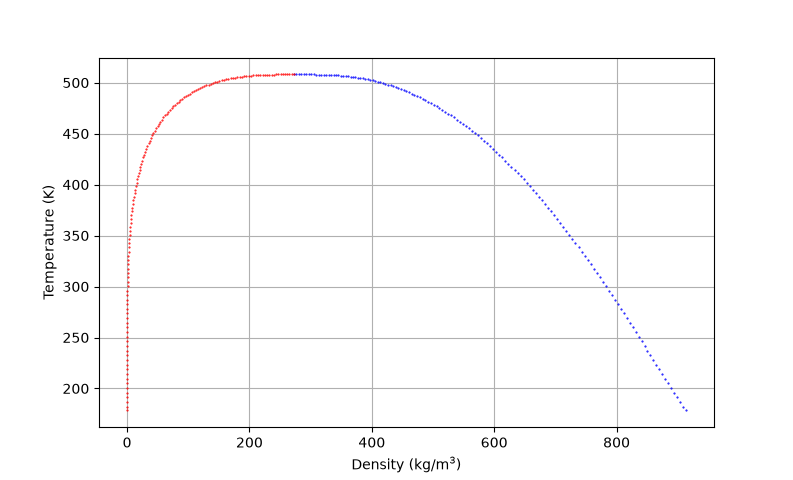
\includegraphics[width=0.97\linewidth]{figures/sattable}
\caption{Points of the saturation table automatically generated by \texttt{mp2} for acetone.}\label{fig:mp:sattable}
\end{figure}

\textbf{Constructing the general property table} requires a rectangular grid of temperature and density values.  The grid is constructed automatically from the saturation curve using a series of rules:
\begin{enumerate}
\item Density and temperature arrays must be in ascending order.
\item No step between any two adjacent values may be larger than a threshold (set in software).
\item The temperature and density arrays must span between their respective minima and maxima.
\item For each temperature below the critical temperature, the density array must be values corresponding precisely to the liquid and vapor saturation densities at that temperature.
\item For each density between the vapor and liquid triple point densities, the temperature array must contain a temperature corresponding precisely to the corresponding saturation temperature.
\end{enumerate}
To obey these rules, it is essential that the saturation table is already available.

From the resulting temperature and density grid values, all properties are evaluated in two-dimensional arrays, so that
\begin{align}
f_{i,j} \equiv f(T_i, \rho_j)
\end{align}

This approach has some very useful consequences.  Firstly, if the critical temperature is found at index, \texttt{i}, and the critical density is found at density index, \texttt{j}.  It is always trivial to identify grid points precisely on the saturation line.  If we were to move $k$ indices below the critical temperature,
\begin{align}
T_s &= T_{i-k}\\
\rho_L &= \rho_{j+k}\\
\rho_V &= \rho_{j-k}
\end{align}

Also, it naturally produces a high density of grid lines in regions where the saturation curves cause properties to be very steep.  Figure \ref{fig:mp:eTd} shows the internal energy table automatically generated for acetone.  There is a tight grouping of temperature grid lines near the critical point, but there is also a remarkably sharp vertical slope under ``the dome'' near the vapor line caused by the severely dissimilar densities between liquids and vapors far below the critical point.  It only takes a small amount of vapor to significantly drop the density, while adding relatively little to the mixture's energy.  It is not until the density has diminished to a tiny fraction (often around 0.2\% or so) of its liquid value that the higher vapor energy dominates.  Note that this grid generation strategy naturally densely populates this region with gridlines, producing a well formed, though nearly vertical surface.

\begin{figure}
\centering
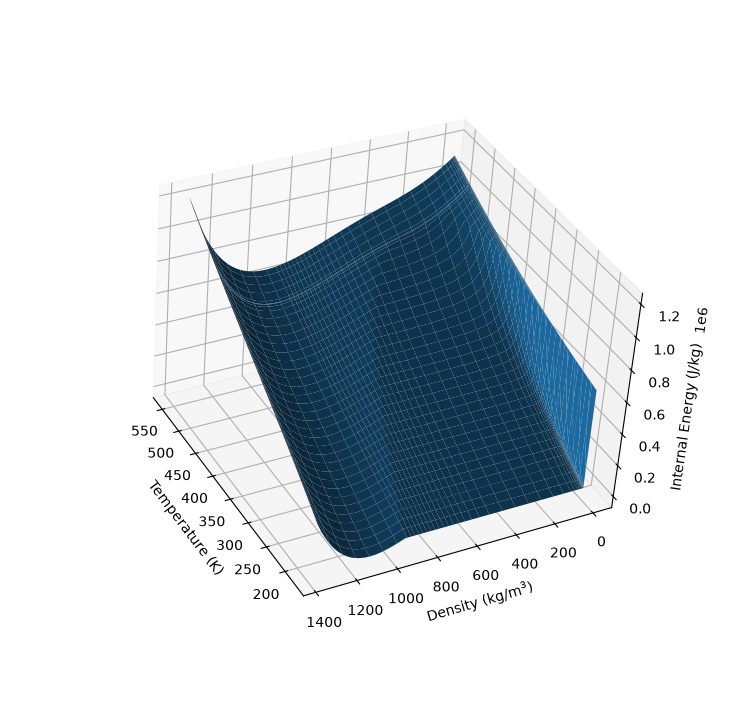
\includegraphics[width=0.97\linewidth]{figures/eTd}
\caption{Internal energy plotted against temperature and density with the grid values automatically generated by \texttt{mp2}.}\label{fig:mp:eTd}
\end{figure}

When any properties other than temperature and/or density are used to reference the state, the tables are used to produce an initial guess for the $T,\rho$ state values that are quite close to the actual solutions.  This relieves \texttt{mp2} of the burden of numerically robust iteration solved by the \texttt{mp1.hybrid1()} algorithm (see Section \ref{sec:num:hybrid1}), so Newton-Rhapson root polishing can be used.

This has quite a few benefits over the approach in \texttt{mp1}:


The development of the \texttt{mp2} class is essential to the expansion of the \PM\ multi-phase data offerings, since many authors who publish coefficients for the Span and Wagner models do not also publish saturation line curves.  This proved quite limiting when attempting to broaden the number of multi-phase substance models.

\subsection{The \texttt{mp1} class}

The \texttt{mp1} class is the older of the two multi-phase classes in \PM.  It 

Many original sources for equation-of-state models include polynomial fits for saturation properties that are so accurate, they can even be implemented without applying the Maxwell criteria.  When these are used as initial guesses, the Maxwell criteria are simply used to ``polish'' the solution to agree more precisely with the equation of state.  As of version 2.4.5, an inner routine, \texttt{\_ds()}, is provided that implements the Maxwell criterion, but saturation property methods do not yet implement it.  At the time of this writing, it is planned to transition in version 2.4.6.

In many sources, formulae are provided for
\begin{itemize}
\item liquid saturation density given temperature,
\item vapor saturation density given temperature,
\item saturation pressure given temperature.
\end{itemize}
From them, all other properties can be obtained along the saturation line.  The \texttt{mp1} class exposes these properties through methods: \texttt{ds}, \texttt{ps}, \texttt{Ts} (not to be confused with \verb|T_s|), \texttt{es}, \texttt{hs}, and \texttt{ss}.  All of these depend on the three basic empirical formulae.

These formulae are calculated from dimensionless temperature, 
\begin{align}
\theta = \frac{T}{T_c},
\end{align}
which is the inverse of $\tau$.  Each of the formulae for a saturation property, $p$, take one of four types:

{\bf 0. A polynomial on $\theta$} 
\begin{align}
p(\theta) = \sum_k c_k \theta^{a_k}
\end{align}
This form is commonly used for liquid-solid saturation lines (not yet implemented in version 2.1.0).

{\bf 1. A polynomial on $1-\theta$}
\begin{align}
p(\theta) = \sum_k c_k (1-\theta)^{a_k}
\end{align}
This form is usually used for the saturation pressure.

{\bf 2. An exponential of a polynomial on $1-\theta$}
\begin{align}
p(\theta) = \exp \left( \sum_k c_k (1-\theta)^{a_k} \right)
\end{align}
This form is usually used for the liquid saturation density.

{\bf 3. An exponential of a polynomial on $1-\theta$ with a $1/\theta$ multiplier}
\begin{align}
p(\theta) = \exp \left( \frac{1}{\theta} \sum_k c_k (1-\theta)^{a_k} \right)
\end{align}
This form is usually used for the vapor saturation density.

In data, there are three groups that are used to define the saturation pressure and densities.
\begin{lstlisting}[language=Python]
"PSgroup" : {
    "fn" : <fn index>,
    "pscale" : <p scale>,
    "Tscale" : <T scale>,
    "coef" : <polynomial coefficients>
}

"DSLgroup" : {
    "fn" : <fn index>,
    "dscale" : <d scale>,
    "Tscale" : <T scale>,
    "coef" : <polynomial coefficients>
}

"DSVgroup" : {
    "fn" : <fn index>,
    "dscale" : <d scale>,
    "Tscale" : <T scale>,
    "coef" : <polynomial coefficients>
}
\end{lstlisting}

The \texttt{fn} parameter is an index (0-3) that selects the form of the formula to use.  The \texttt{pscale} and \texttt{dscale} parameters are used to re-scale the dimensionless property calculated by the selected formula.  The \texttt{Tscale} parameter is used to normalize temperature to calculate $\theta$.  Finally, \texttt{coef} is a polynomial coefficient list described in Section \ref{sec:num:poly1}.


\section{Sources implemented}
Table \ref{tab:mp:source} lists the multi-phase models currently implemented in \PM\ as of version 2.2.0.  Entries marked with an asterisk were not yet complete for the 2.2.0 release, but are planned to be implemented later.

\begin{table}
\centering
\caption{Sources for multi-phase data used in \PM.  Substances with a * were not yet implemented in version 2.2.0, but they are planned for a later release.}\label{tab:mp:source}
\begin{tabular}{|ccc|}
\hline
Argon* & Ar & \cite{tegeler:1999}\\
Carbon dioxide & CO$_2$ & \cite{span:1994}\\
Deuterium* & D$_2$ & \cite{richardson:2013}\\
Hydrogen* & H$_2$ & \cite{leachman:2009}\\
Nitrogen & N$_2$ & \cite{span:2000}\\
Oxygen & O$_2$ & \cite{stewart:1991}\\
Water & H$_2$O & \cite{iapws:2014}\\
R-125* & C$_2$HF$_5$ & \cite{piao:1998}\\
R-134a & C$_2$H$_2$F$_4$ & \cite{tilner:1994}\\
R-143a* & C$_2$H$_2$F$_3$ & \cite{lemmon:2000}\\
R-245fa* & C$_3$H$_3$F$_5$ & \cite{akasaka:2015}\\
R-1234yf* & C$_3$H$_2$F$_4$ & \cite{richter:2011}\\
R-1234ze & C$_3$H$_2$F$_4$ & \cite{thol:2016}\\
\hline
\end{tabular}
\end{table}
